\documentclass[addpoints]{exam}

\usepackage{amsmath}
\usepackage[utf8]{inputenc}
\usepackage{tikz}

\usetikzlibrary{shapes.geometric, arrows, fit, matrix, positioning}

\begin{document}

\section*{Exame 2020/2021 (Época Normal)}

\begin{questions}

\question Pergunta 1

a. A connectionless reliable service.

\question Pergunta 2

d. 200 kbits/s

\question Pergunta 3

c. FERa $>$ FERb

\question Pergunta 4

b. !I(1).SW

\question Pergunta 5

e. $\lambda$

\question Pergunta 6

d. TDM $>$ Slotted Aloha $>$ Aloha

\question Pergunta 7

b. MAC address of RT.port0

\question Pergunta 8

b. forwarded to port 3

\question Pergunta 9

d. 6 ms 

\question Pergunta 10

a. information about all the nodes

\question Pergunta 11

$R = 600 kbits/s = 600000 bits/s$

$T_{p} = 40 ms = 0.04 s$

$L = 300 bytes = 2400 bits$

$BER = 0.0001$

$
P_{e} = 1 - (1 - BER)^{L}
      = 1 - (1 - 0.0001)^{2400}  
      = 0.213382
$

$
T_{f} = \frac{L}{R}
      = \frac{2400}{600000}
      = 0.004
$

$
a = \frac{T_{p}}{T_{f}}
  = \frac{0.04}{0.004}
  = 10
$

$
S = \frac{1 - P_{e}}{1 + 2a \cdot P_{e}}
  = \frac{1 - 0.213382}{1 + 2 \cdot 10 \cdot 0.213382}
  = 0.14933
  \approx 15\%
$

\question Pergunta 12

$
S = \frac{W \cdot (1 - P_{e})}{1 + 2a}
  = \frac{16 \cdot (1 - 0.213382)}{1 + 2 \cdot 10}
  = 0.6
$

$
R_{max} = S \cdot R
        = 0.6 \cdot 600
		= 360 kbits/s
$

\question Pergunta 13

$BER = 0$

$
S = \frac{W}{1 + 2a}
\iff 1 = \frac{16}{1 + 2 \frac{40 \cdot 10^{-3}}{\frac{L}{600000}}}
\iff 15L = 80 \cdot 10^{3} \cdot 6 \cdot 10^{5}
\iff L = 3200 bits
       = 400 bytes
$

\question Pergunta 14

$\rho = 0.8$

$C = 100 Mbits/s = 10^{8} bits/s$

$L = 10^{4} bits$

$
\mu = \frac{C}{L} 
	= \frac{10^{8}}{10^{4}} 
	= 10000
$

$
\lambda = \rho \cdot \mu 
		= 0.8 \cdot 10000
		= 8000
$

$
\lambda_{port} = \frac{\lambda}{N_{ports}}
			   = \frac{8000}{10}
			   = 800
$

\question Pergunta 15

$B = 4$ (number of buffers)

$
P(B) = \frac{(1 - \rho)\rho^{B}}{1 - \rho^{B + 1}}
     = \frac{(1 - 0.8) \cdot 0.8^{4}}{1 - 0.8^{5}}
     = 0.121847
$

$
P(\bar{B}) = 1 - P(B) = 1 - 0.121847 \approx 88\%
$

\question Pergunta 16

$
N = \frac{\rho}{1 - \rho} 
  = \frac{0.8}{0.2} 
  = 4
$

$
N' = N - 1 = 3
$

$
T_{w} = N' \cdot T_{s} 
	  = 3 \cdot \frac{1}{\mu} 
	  = \frac{3}{10000} 
	  = 0.0003 s
	  = 300 \mu s
$

\question Pergunta 17

\begin{center}
	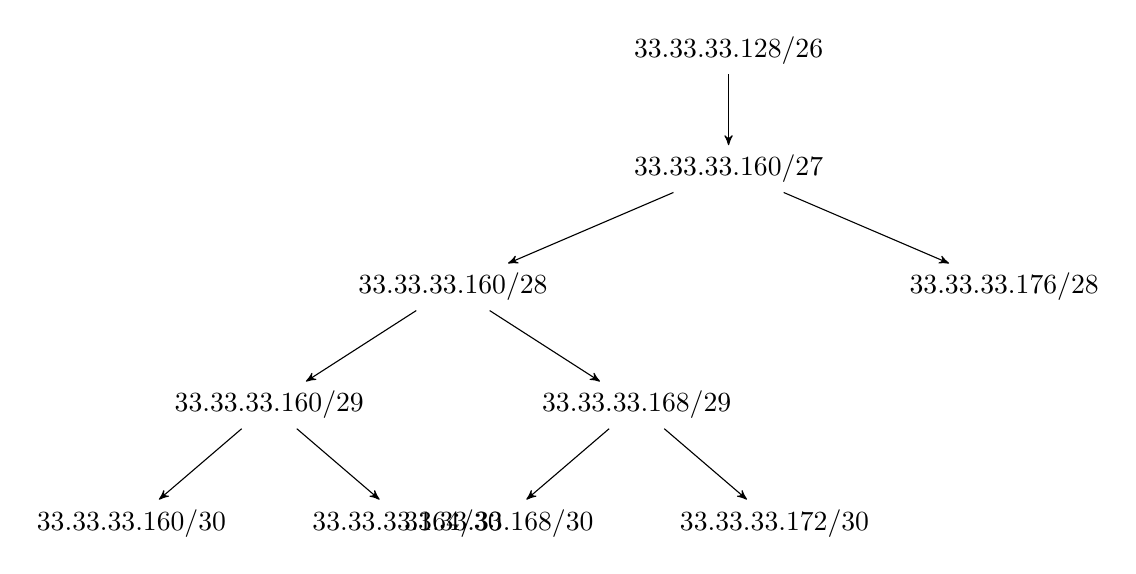
\begin{tikzpicture}[->,>=stealth',level/.style={sibling distance = 14cm/#1,
		level distance = 1.5cm}, transform shape]
		\node {33.33.33.128/26}
		child
		{
			node {33.33.33.160/27} 
			child {
				node {33.33.33.160/28} 
				child {
					node {33.33.33.160/29} 
					child {
						node {33.33.33.160/30} 
					}
					child {
						node {33.33.33.164/30} 
					}
				}
				child {
					node {33.33.33.168/29} 
					child {
						node {33.33.33.168/30} 
					}
					child {
						node {33.33.33.172/30} 
					}
				}
			}
			child {
				node {33.33.33.176/28} 
			}
		}
	;
	\end{tikzpicture}
\end{center}

33.33.33.176/28

\question Pergunta 18

33.33.33.159

\question Pergunta 19

33.33.33.173

\question Pergunta 20

a. R4

\end{questions}

\end{document}
